\chapter{Prozessmodelle}\label{sec:chapter2}

In Kapitel 2 werden grundlegende Konzepte des Software Engineering vorgestellt, welche notwenidg sind, um den Inhalt dieser Arbeit besser zu verstehen. Zunächst wird in Kapitel 2.1 der Begriff Software Engineering definiert und die Ziele, der Prozess und die Prinzipien des Software Engineering werden erläutert. Weiterhin wird in Kapitel 2.2 der Begriff Softwareprozessmodell erklärt. Hierbei werden Software-Projekttypen sowie schwergewichtige und leichtgewichtige Prozessmodelle beschrieben. Anschließend gibt es eine Einführung in die drei Softwareprozessmodelle Scrum, Open Unified Process und V-Modell-XT.

\section{Software Engineering}\label{sec:chapter2: Software Engineering}
Heutzutage werden immer mehr Systeme von Software kontrolliert. Dies macht Software Engineering zu einer der bedeutendsten Technologien \cite{Puntambekar2007}.
Unter Software versteht man laut Duden die "Gesamtheit aller Programme, die auf einem Computer eingesetzt werden können". Das Wort Engineering, welches sich laut Duden von dem lateinischen Wort Ingenium (=[schöpferische] Begabung; Erfindungsgabe) ableitet, wird heutzutage mit Ingenieurwesen, bzw. technische Entwicklung übersetzt. Software Engineering umfasst somit die Gesamtheit der Aktivitäten zur Analyse, Konzeption, Entwicklung und Implementierung einer softwaretechnischen Lösung \cite{Specker1998}.
Software Engineering besteht aus mehreren Schichten (Abbildung \ref{fig:SchichtenSE}):

\begin{figure}[htp]
\begin{center}
  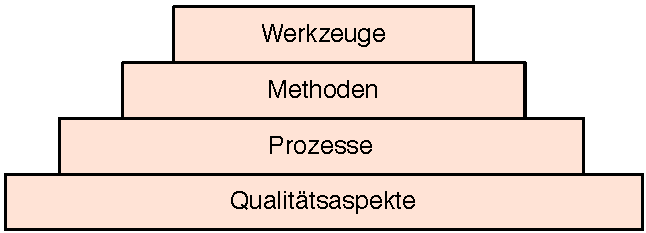
\includegraphics[width=.5\linewidth]{SELayer} %pdf, jpg, png...
  \caption{Schichten des Software Engineering \cite{Puntambekar2007}}
  \label{fig:SchichtenSE}
\end{center}
\end{figure}

Somit sind für Software Engineering ein diszipliniertes Qualitätsmanagement sowie eine Prozessschicht vorhanden, um die termingerechte Ablieferung von Software zu gewährleisten. In der Methoden-Schicht wird sodann die Implementierung unter Zuhilfenahme von Requirementanalysen, Design und Programmierung durchgeführt. Hierbei werden Werkzeuge zur Automatisierung in SoftwareDokumenteprozessen benutzt \cite{Puntambekar2007}. 

\subsection{Ziele, Prozess und Prinzipien des Software Engineering}

Das Hauptziel in der Software Entwicklung ist, dass die Lösungen mit den Anforderungen übereinstimmen. Vollständige und konsistente Anforderungserhebungen sind, insbesondere für große Systeme, selten. Sowohl die Nutzer, als auch die Entwickler haben ein oftmals unvollständiges Verständnis des eigentlichen Problems und erheben somit ihre Anforderungen erst während der Entwicklung. Somit muss man mit Änderungen der Anforderungen an ein System während dessen Entwicklung rechnen. Aus diesem Grund ist es wichtig, Ziele beim Software Engineering zu haben, um die Auswirkungen solcher Änderungen einzudämmen \cite{Booch1993}.
Abbildung  \ref{fig:Wuerfel} zeigt die von \cite{ross1975software} definierten Ziele, Prinzipien und den Prozess des Software Engineering, welche nachfolgend genauer erläutert werden: 

\begin{figure}[htp]
\begin{center}
  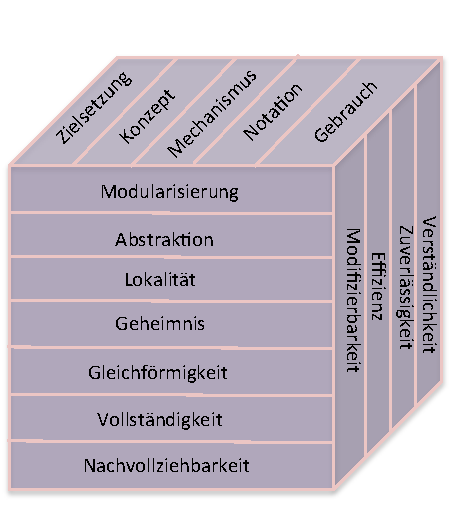
\includegraphics[width=0.6\linewidth]{Wuerfel} %pdf, jpg, png...
  \caption{Ziele, Prozess und Prinzipien des Software Engineering  \cite{ross1975software}}
  \label{fig:Wuerfel}
\end{center}
\end{figure}

\subsubsection{Prinzipien des Software Engineering}


 Das \textit{Modluarisierungsprinzip} gibt eine geeignete Strukturierung für Softwaresysteme an. Das \textit{Abstraktionsprinzip} soll dabei helfen, sich von unwichtigen Details, welche für die zu entwickelnde Lösung irrelevant sind, zu lösen. Das \textit{Geheimnisprinzip} bezieht sich auf das Definieren und Durchsetzen von Zugriffsbeschränkungen. Das \textit{Lokalitätsprinzip} verlangt das räumlich zusammenhängende Ablegen von zusammengehörenden Informationen. Konsistenz wird durch das \textit{Gleichförmigkeitsprinzip} gewährleistet. Durch das \textit{Vollständigkeitsprinzip} wird sichergestellt, dass nichts vergessen wurde. Das Prinzip der \textit{Nachvollziehbarkeit} stellt sicher, dass Informationen, welche zur Überprüfung der Korrektheit benötigt werden, detailliert dargelegt werden \cite{ross1975software}.
 
 \subsubsection{Prozess des Software Engineering}

Wie Abbildung  \ref{fig:Wuerfel} entnommen werden kann, besteht der Prozess des Software Engineering aus 5 Schritten: Im ersten Schritt \textit{Zielsetzung} werden die Anforderungen an ein System festgelegt. Anschließend erfolgt im Schritt \textit{Konzept} die Ableitung der Software-Architektur, um die zuvor erhobenen Anforderungen zu erfüllen. Des Weiteren werden die Komponenten des Software-Systems festgelegt. Im dritten Schritt \textit {Mechanismus} erfolgt sodann die Implementierung des Software-Systems. Im darauffolgenden Schritt \textit{Notation} wird die Kommandosprache definiert, die ein Benutzer verwendet, um die Funktionalitäten des Software-Systems aufzurufen. Im letzten Schritt \textit{Gebrauch} muss noch die Bedienung des Systems, z.B. in Form eines Benutzerhandbuches, beschrieben werden \cite{ross1975software}.
  \subsubsection{Ziele des Software Engineering}

\textit{Modifizierbarkeit} ist das wohl schwierigste Ziel des Software Engineering. Hierbei geht es darum, dass es manchmal notwendig ist, Teile des zu entwickelnden Systems zu ändern, während andere Teile unverändert bleiben, aber dennoch das gewünschte neue Ergebnis erreicht wird. Auf die \textit{Effizienz} der jeweiligen Aktivitäten sollte immer geachtet werden, da dieses Ziel des Software Engineering häufig vernachlässigt wird. Bei dem Ziel \textit{Zuverlässigkeit} geht es darum, einerseits Fehler bei der Konzeption, im Design und der Implementierung zu vermeiden, andererseits muss auch Fehlverhalten bei der Ausführung und der Leistung verhindert werden.
 
\section{Softwareprozessmodelle}\label{sec:chapter.2: Softwareprozessmodelle}

Für das Verständnis, die Schaffung oder Unternehmung von etwas Großem, fertigen Menschen in der Regel ein vereinfachtes Bild davon an, bzw. nehmen Maß, fertigen eine Skizze oder einen Plan an oder orientieren sich an einem Vorbild, bzw. bauen sich eines. Dies geschieht normalerweise mit Papier und Schreibzeug, anderen Materialien oder einem Computer. Besonders für die Lösung von komplexen wissenschaftlichen Problemen oder für die Erfüllung großer Führungs- und Konstruktionsaufgaben ist dies unumgänglich \cite{Hesse2008}. \newline
Hierbei stützten sie sich auf Modelle, welche als Stellvertreter für die Sache, die verstanden, geschaffen, unternommen oder betrieben werden soll, angesehen werden kann \cite{Hesse2008}. \newline
Insbesondere die heutzutage von Softwareentwicklern zu erstellenden Softwareprodukte zeichnen sich durch ein hohes Maß an Komplexität und Umfang aus. Neben den Erwartungen von Kunden hinsichtlich Qualität müssen Softwaresysteme ebenfalls termingerecht und innerhalb eines vorgegebenen Budgetrahmens erstellt werden. Effektive und effiziente Softwareprozessmodelle gewinnen somit immer mehr Bedeutung \cite{Grechenig2010}.
Modell leitet sich von dem lateinischen Begriff  \glqq modelus \grqq
ab und kann mit  \glqq Regel, Form, Muster, Vorbild \grqq übersetzt werden \cite{Hesse2008}. 
Der Begriff Prozess stammt von dem lateinischen Wort "processus" ' ab und lässt sich mit "Fortgang oder Verlauf" ' übersetzen \cite{koch2011, Staud2006}. \newline 
Ein Softwareprozess stellt eine Abfolge von Schritten dar, welche zur Herstellung von Software notwendig sind \cite{Mishra2012, Stoerrle2005}. Mit Hilfe eines Softwareprozessmodelles lässt sich der organisatorische Rahmen zur Herstellung von Software beschreiben \cite{Koelmel2000}. Ein Softwareprozessmodell stellt somit ein Modell für die Entwicklung eines Software-Systems dar \cite{Hanser2010}. Die einzelnen Abschnitte eines Softwareprozesses werden hierbei als Phasen bezeichnet \cite{Stoerrle2005}. Diese werden unterscheiden in (Abbildung \ref{fig:SEProzess}):

\begin{figure}[htp]
\begin{center}
  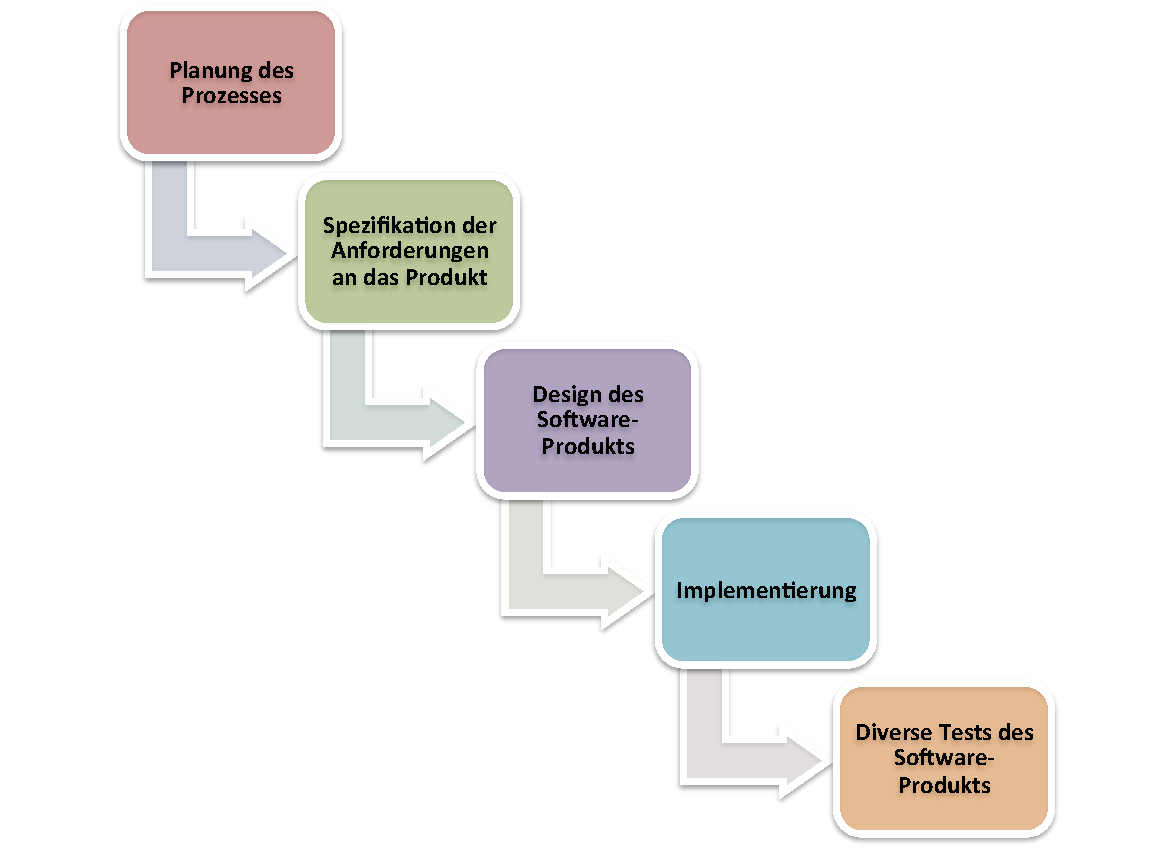
\includegraphics[width= 0.8\linewidth]{Softwareprozess} %pdf, jpg, png...
  \caption{Phasen Softwareprozess nach \cite{Hanser2010}}
  \label{fig:SEProzess}
\end{center}
\end{figure}

In einem Softwareprozessmodell werden nicht nur die durchzuführenden Aktivitäten definiert, sondern auch die Rollen und Qualifikationen der Mitarbeiter, welche die jeweiligen Aktivitäten durchführen sollen, bzw. für diese verantwortlich sind. Des Weiteren werden die während des Entwicklungsprozesses zu erstellenden Dokumente und Unterlagen festgelegt \cite{Hanser2010}.

\subsection{Software-Projekttypen}

Software-Projekte lassen sich in drei Gruppen einteilen (Abbildung \ref{fig:Projekttypen}):

\begin{figure}[htp]
\begin{center}
  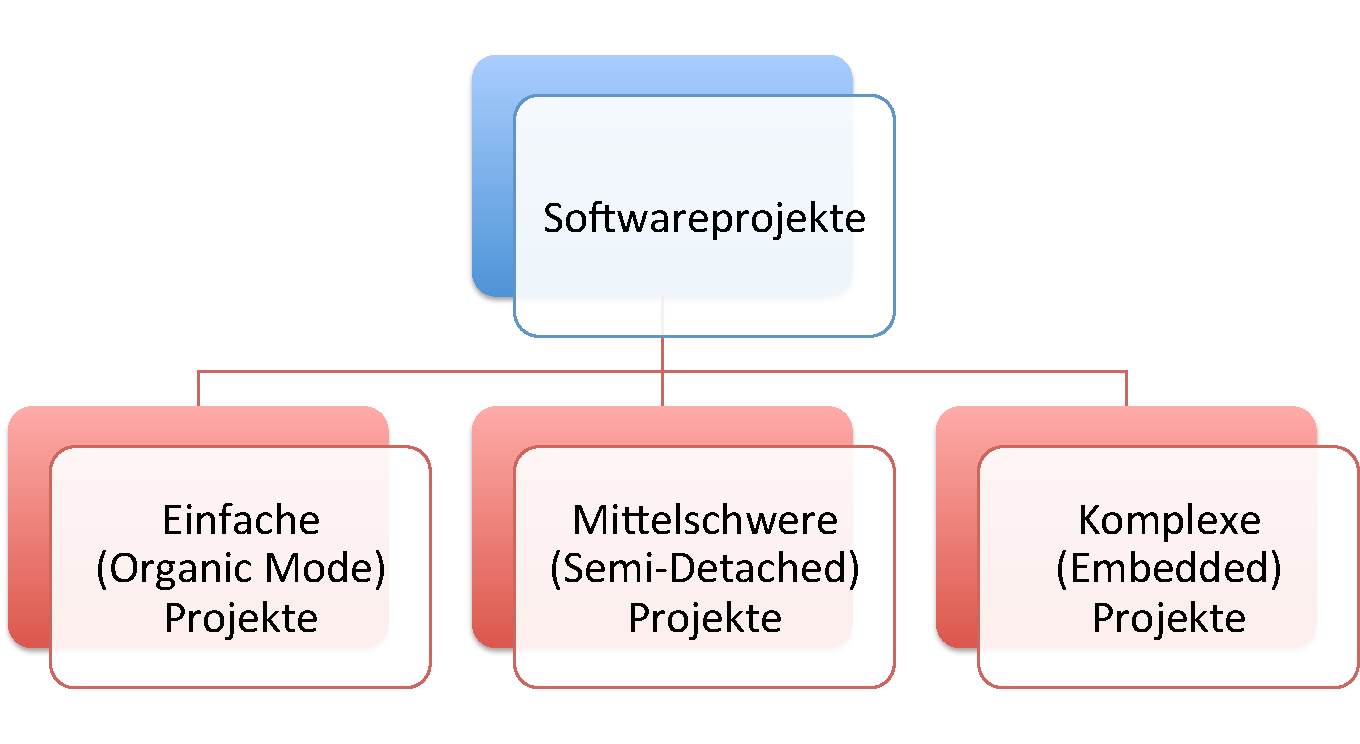
\includegraphics[width= 0.8\linewidth]{Projekttypen} %pdf, jpg, png...
  \caption{Software-Projekttypen nach \cite{Boehm81}}
  \label{fig:Projekttypen}
\end{center}
\end{figure}

Bei den \textit{Einfachen Projekten} sind relativ kleine Teams am Entwicklungsprozess beteiligt und bei den Teammitgliedern besteht räumliche Nähe. Jedes Teammitglied weist eine hohe methodische und fachliche Erfahrenheit auf und kennt sich in dem späteren Einsatzgebiet der Software gut aus. Die Anzahl der Code-Zeilen bei der zu entwickelnden Software ist meist gering \cite{Boehm81, Hanser2010}. \newline
Bei den \textit{Komplexen Projekten} handelt es sich um Software-Projekte, welche in den meisten Fällen stark durch behördliche Auflagen reguliert sind. Die Software muss einerseits eine hohe Zuverlässigkeit aufweisen und andererseits sind nachträgliche Änderungen fast nicht mehr möglich. Im Gegensatz zu den \textit{Einfachen Projekten} ist das Entwicklungsteam hier groß, besteht sowohl aus erfahrenen, als auch aus unerfahrenen Entwicklern und die Anzahl der Code-Zeilen ist ebenfalls groß \cite{Boehm81, Hanser2010}. \newline
Eine Schnittstelle zwischen diesen beiden Projekttypen bilden die \textit{Mittelschweren Projekte}. Hier sind die Software-Entwicklungsteams mittelgroß und bestehen aus erfahrenen und unerfahrenen Mitgliedern. Teilweise sind nicht alle Aspekte des Produktes schon im Vornherein bekannt und die Anzahl der Code-Zeilen ist groß \cite{Boehm81, Hanser2010}.

\subsection{Schwergewichtige und leichtgewichtige Prozessmodelle}

Aus der eben erfolgten Einteilung von Software-Projekten lässt sich eine Einteilung von Software-Prozessmodellen in \textit{leichtgewichtige} und \textit{schwergewichtige Prozessmodelle} ableiten \cite{Hanser2010}. \newline
\textit{Leichtgewichtige Prozessmodelle} eignen sich eher für kleine Teams, bei denen keine detaillierte Anforderungserhebung stattfindet, da die Kommunikation sowohl innerhalb des Teams, als auch mit dem Kunden auf Grund der kleinen Teamgröße gut funktioniert. Da viele Informationen hier informell über kurze Kommunikationswege weitergegeben werden, ist eine ausführliche Dokumentation derer nicht notwendig. Der Einsatz von \textit{leichtgewichtigen Prozessmodellen} eignet sich sehr gut für \textit{einfache Projekte} und teilweise auch für \textit{mittelschwere Projekte}\cite{Hanser2010}. \newline
Eine sehr formale und dokumentenlastige Vorgehensweise kommt bei den \textit{schwergewichtigen Prozessmodellen} zum Einsatz. Es findet eine ausführliche Dokumentation in allen Entwicklungsphasen statt und der Ablauf des Prozesses ist genau vorgegeben. Bei Software-Produkten, welche bei einer möglichen Fehlfunktion Menschenleben in Gefahr bringen, ist beispielsweise eine Vorgehensweise mit einem \textit{schwergewichtigen Prozessmodell} sinnvoll. Ihr Einsatz ist besonders in \textit{schweren Projekten} vorzuziehen, aber auch in \textit{mittelschweren Projekten} \cite{Hanser2010}. \newline













